% Session 6 -- the Stoner criterion.
% Placement: sec. "A criterion for magnetism: the Stoner threshold", right after eq. (6.3).
% Rendered by figures/blender/s06f01_stoner.py, labels in figures/overlays/s06f01_stoner.tex.
\begin{aqmfigure}{fig:s06:stoner}{A graphical reading of the Stoner criterion (6.3). (a) The
self-consistency condition $m=f(m)$, where $f$ is the right-hand side of the zero-temperature gap
equation, drawn here with the shape $\tanh$ for two values of the slope. It is an odd function that
saturates once the bands are fully polarized, and its slope at the origin is exactly $U D(E_F)$. If
this slope is below one, the only crossing with $y=m$ is the trivial solution $m=0$. Once the slope
is above one, a pair of nontrivial solutions $\pm m_0$ appears and the nonmagnetic state becomes
unstable. (b) The resulting order parameter, which stays at zero until $U D(E_F)$ reaches one and
then grows continuously. For this reason, whether a metal becomes magnetic is not decided by $U$
alone but by the \emph{product} of $U$ with the density of states at the Fermi level. This is why
aluminium and lead stay nonmagnetic even with a sizeable Coulomb repulsion, while the narrow $d$
bands of iron and cobalt are clearly above the threshold.}
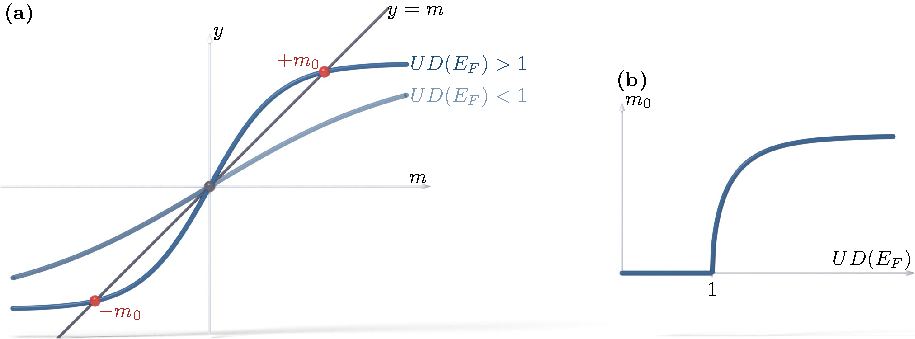
\includegraphics{figures/pdf/s06f01_stoner.pdf}
\end{aqmfigure}
